% Section content template for individual Educative lessons
% This file contains the actual content for a specific section
% Generated from Educative API section content

% Section: Activity Diagram for the Restaurant Management System
% Section ID: 5616451496181760
% Section Slug: activity-diagram-for-the-restaurant-management-system
% Generated: 2025-12-14T12:24:13.691295

Activity diagrams are a great way to visualize the flow of messages from one activity to another in the system. There can be different activity diagrams that we can create for our restaurant management system. In this lesson, we'll create activity diagrams for the following two activities:

\begin{itemize}
\item
\protect\phantomsection\label{ISroyW0i2x3dOFospai-Y}
Activities for the walk-in customer to place an order
\item
\protect\phantomsection\label{-QVzWTDefKPjpCeGP4gHp}
\textbf{Activity challenge:} Generate a bill and process the payment.
\end{itemize}

\subsection{Place the order}\label{KlJr8r4SjFXwZkWstM52i}
\\
The following are the states and actions that will be involved in this activity diagram.

\subsubsection{States}\label{mUmkuR8KlRUo7ZYtAKarH}
\\
\textbf{Initial state:} A customer arrives at the restaurant and asks for a table.
\\
\textbf{Final state:} The customer successfully placed a food order.

\subsubsection{Actions}\label{Jer-vjNeCJZKMLF4olKAc}
\\
The customer arrives at the restaurant's reception and requests a table. The receptionist checks for table availability. If a table is available, the customer is seated. If no table is available, the customer waits until one becomes free.
\\
Once the customer is seated, the server approaches with the menu. The customer reviews the menu and decides what to order. The waiter then takes the customer's order.
\\
Based on the order above, the activity diagram of the table booking and the food order is shown below:

\begin{figure}[htbp]
 \centering
 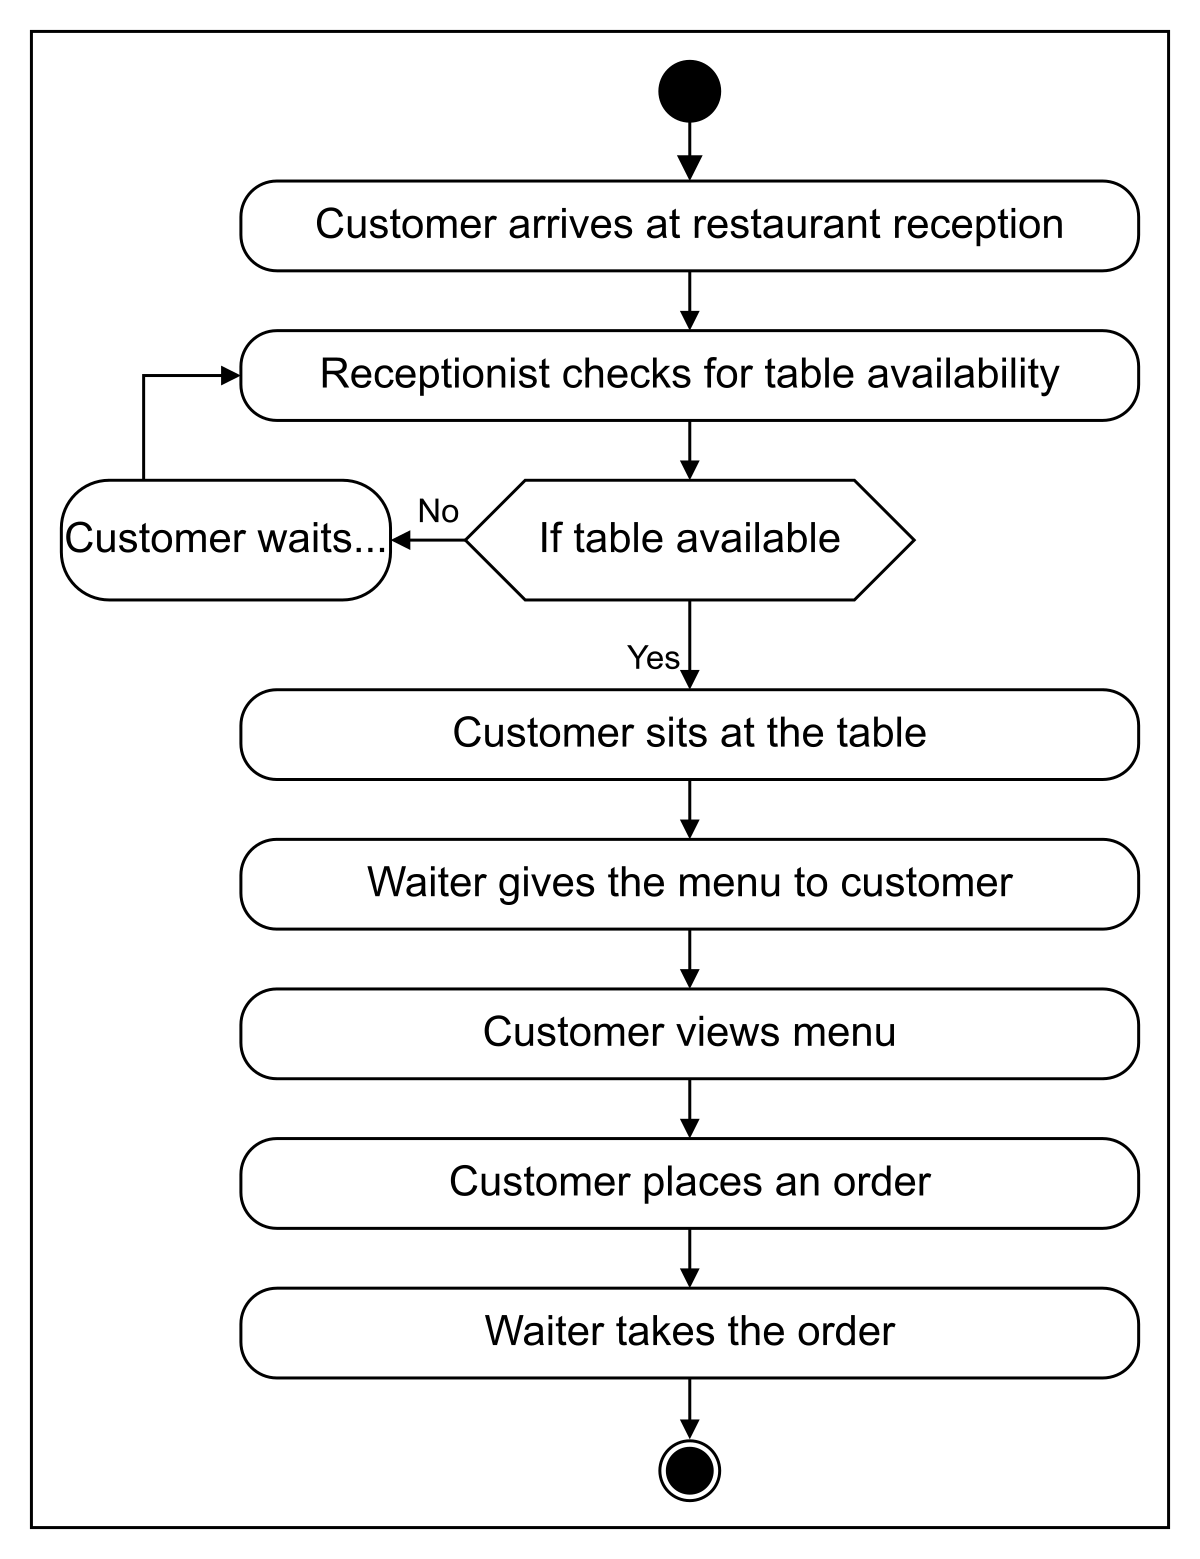
\includegraphics[width=0.5\textwidth]{Images/chapter_21/section_5616451496181760/6232260691755008.png}
 \caption{The activity diagram for placing the order}
\end{figure}

\subsection{Activity challenge: Billing and payment}\label{qQ8UiLDWEEf6Cnibbq9TJ-2}
\\
Let's create an activity diagram for a customer to pay the bill.
\\
A skeleton of the activity diagram is given below.

\begin{figure}[htbp]
 \centering
 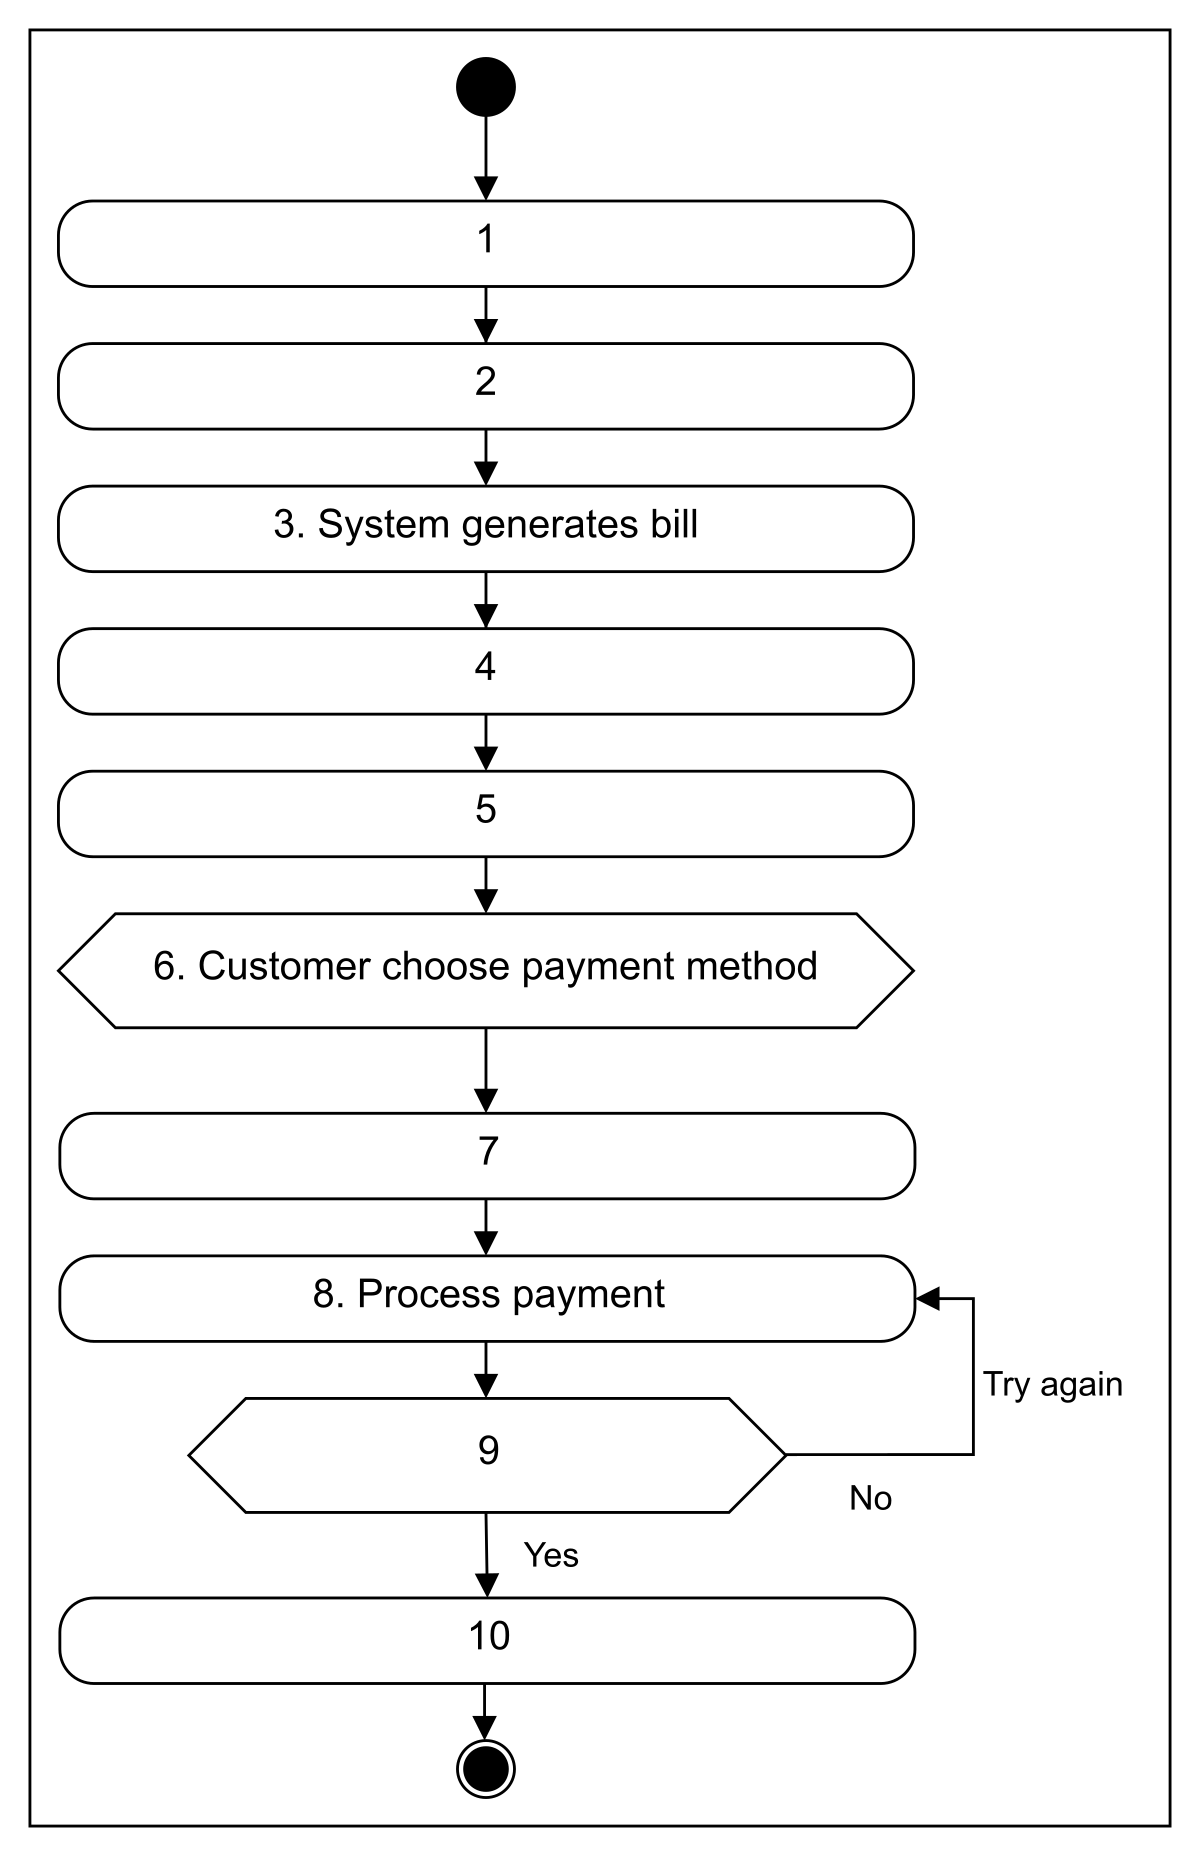
\includegraphics[width=0.5\textwidth]{Images/chapter_21/section_5616451496181760/4837910195863552.png}
 \caption{The activity diagram for order cancellation}
\end{figure}

Notice that the actions in the diagram above are numbered from 1 to 10. The slots shown below represent the activities. Can you rearrange the slots below in the correct order they should appear in the activity diagram above?
\begin{quote}
\textbf{Note:} If you're stuck, click the ``Show Solution'' button.
\end{quote}

\textit{Component type 'Permutation' not yet supported.}

Alternatively, click the ``Show complete diagram'' button below to see the complete activity diagram.

We've looked at some of our restaurant management system's activity diagrams. In the next lesson, we will present the code for our designed classes in some of the most popular languages.

% End of section content